\documentclass[12t, a4paper]{article}
\usepackage{CJKutf8}
\usepackage[left=2cm, right=2cm, top=3cm, bottom=2.5cm]{geometry}
\usepackage[nodayofweek,level]{datetime}
\usepackage{comment}

%..This section controls the header-footer layout of the document
\usepackage{fancyhdr}
\pagestyle{fancy}
\lhead{Computer Network (NTU CSIE, Fall 2017)}
\chead{}
\rhead{Homework \#2}
\renewcommand{\headrulewidth}{0.4pt}

%..This section controls the title layout
\title{\vspace{-6ex}\bf{\LARGE{Homework \#2}}} 
\author{資工三\space B04902009\space蕭千惠} % \footnote{blablabla} 
\date{\vspace{-2ex}\today\vspace{-3ex}}
%{\formatdate{21}{2}{2017}}

%.. Customize section numbering
\renewcommand\thesubsection{(\arabic{subsection})}
\usepackage{color}

%.. Insert graph
\usepackage{graphicx}
% \includegraphics[width=\textwidth, height=10cm, keepaspectratio=true]{pic.jpg}

%.. indent
\usepackage{indentfirst}
\setlength{\parindent}{2em}

%.. hyperlink / url
\usepackage[hyphens]{url}
\usepackage{hyperref}
\hypersetup{
    colorlinks=true,
    linkcolor=blue,
    filecolor=magenta,      
    urlcolor=blue,
}
\urlstyle{same}
%%\url{url}
%%\herf{url}{words to show}

%.. change font size
\usepackage{type1cm}

%.. change enumerate label
\usepackage{enumitem}
%%\begin{enumerate}[label=(\alph*)]  //(a) (b) (c)
%%\begin{enumerate}[label=(\Alph*)]  //(A) (B) (C)
%%\begin{enumerate}[label=(\roman*)] //(i) (ii) (iii`')

%.. define tab
\newcommand\tab[1][1cm]{\hspace*{#1}}


%.. Content
\begin{document}
	\begin{CJK}{UTF8}{bkai}
	\maketitle\thispagestyle{fancy}
	\fontsize{12pt}{16pt} \selectfont	
	
	\section*{How to execute the program?}
		\subsection*{IP \& Port}
		\noindent sender:\\
		\tab	ip: 127.0.0.1\\
		\tab	port: 5000\\
		agent:\\
		\tab	ip: 127.0.0.1\\
		\tab	port: 5001\\
		receiver:\\
		\tab	ip: 127.0.0.1\\
		\tab	port: 5002\\

		\subsection*{Compile}
		\noindent Language: C\\
		\texttt{gcc sender.c -o sender}\\
		\texttt{gcc agent.c -o agent}\\
		\texttt{gcc receiver.c -o receiver}

		\subsection*{Execute}
		\noindent \texttt{./sender <agent\_ip> <agent\_port> <read\_file\_path>}\\
		\texttt{./agent <sender\_ip> <sender\_port> <receiver\_ip> <receiver\_port>}\\
		\texttt{./receiver <agent\_ip> <agent\_port> <write\_file\_path>}\\

		\subsection*{Example}
		\noindent ./sender 127.0.0.1 5001 file.txt\\
		./agent 127.0.0.1 5000 127.0.0.1 5002 0.2\\
		./receiver 127.0.0.1 5001 output.txt\\

	\section*{Program structure}
		\subsection*{Sender}
			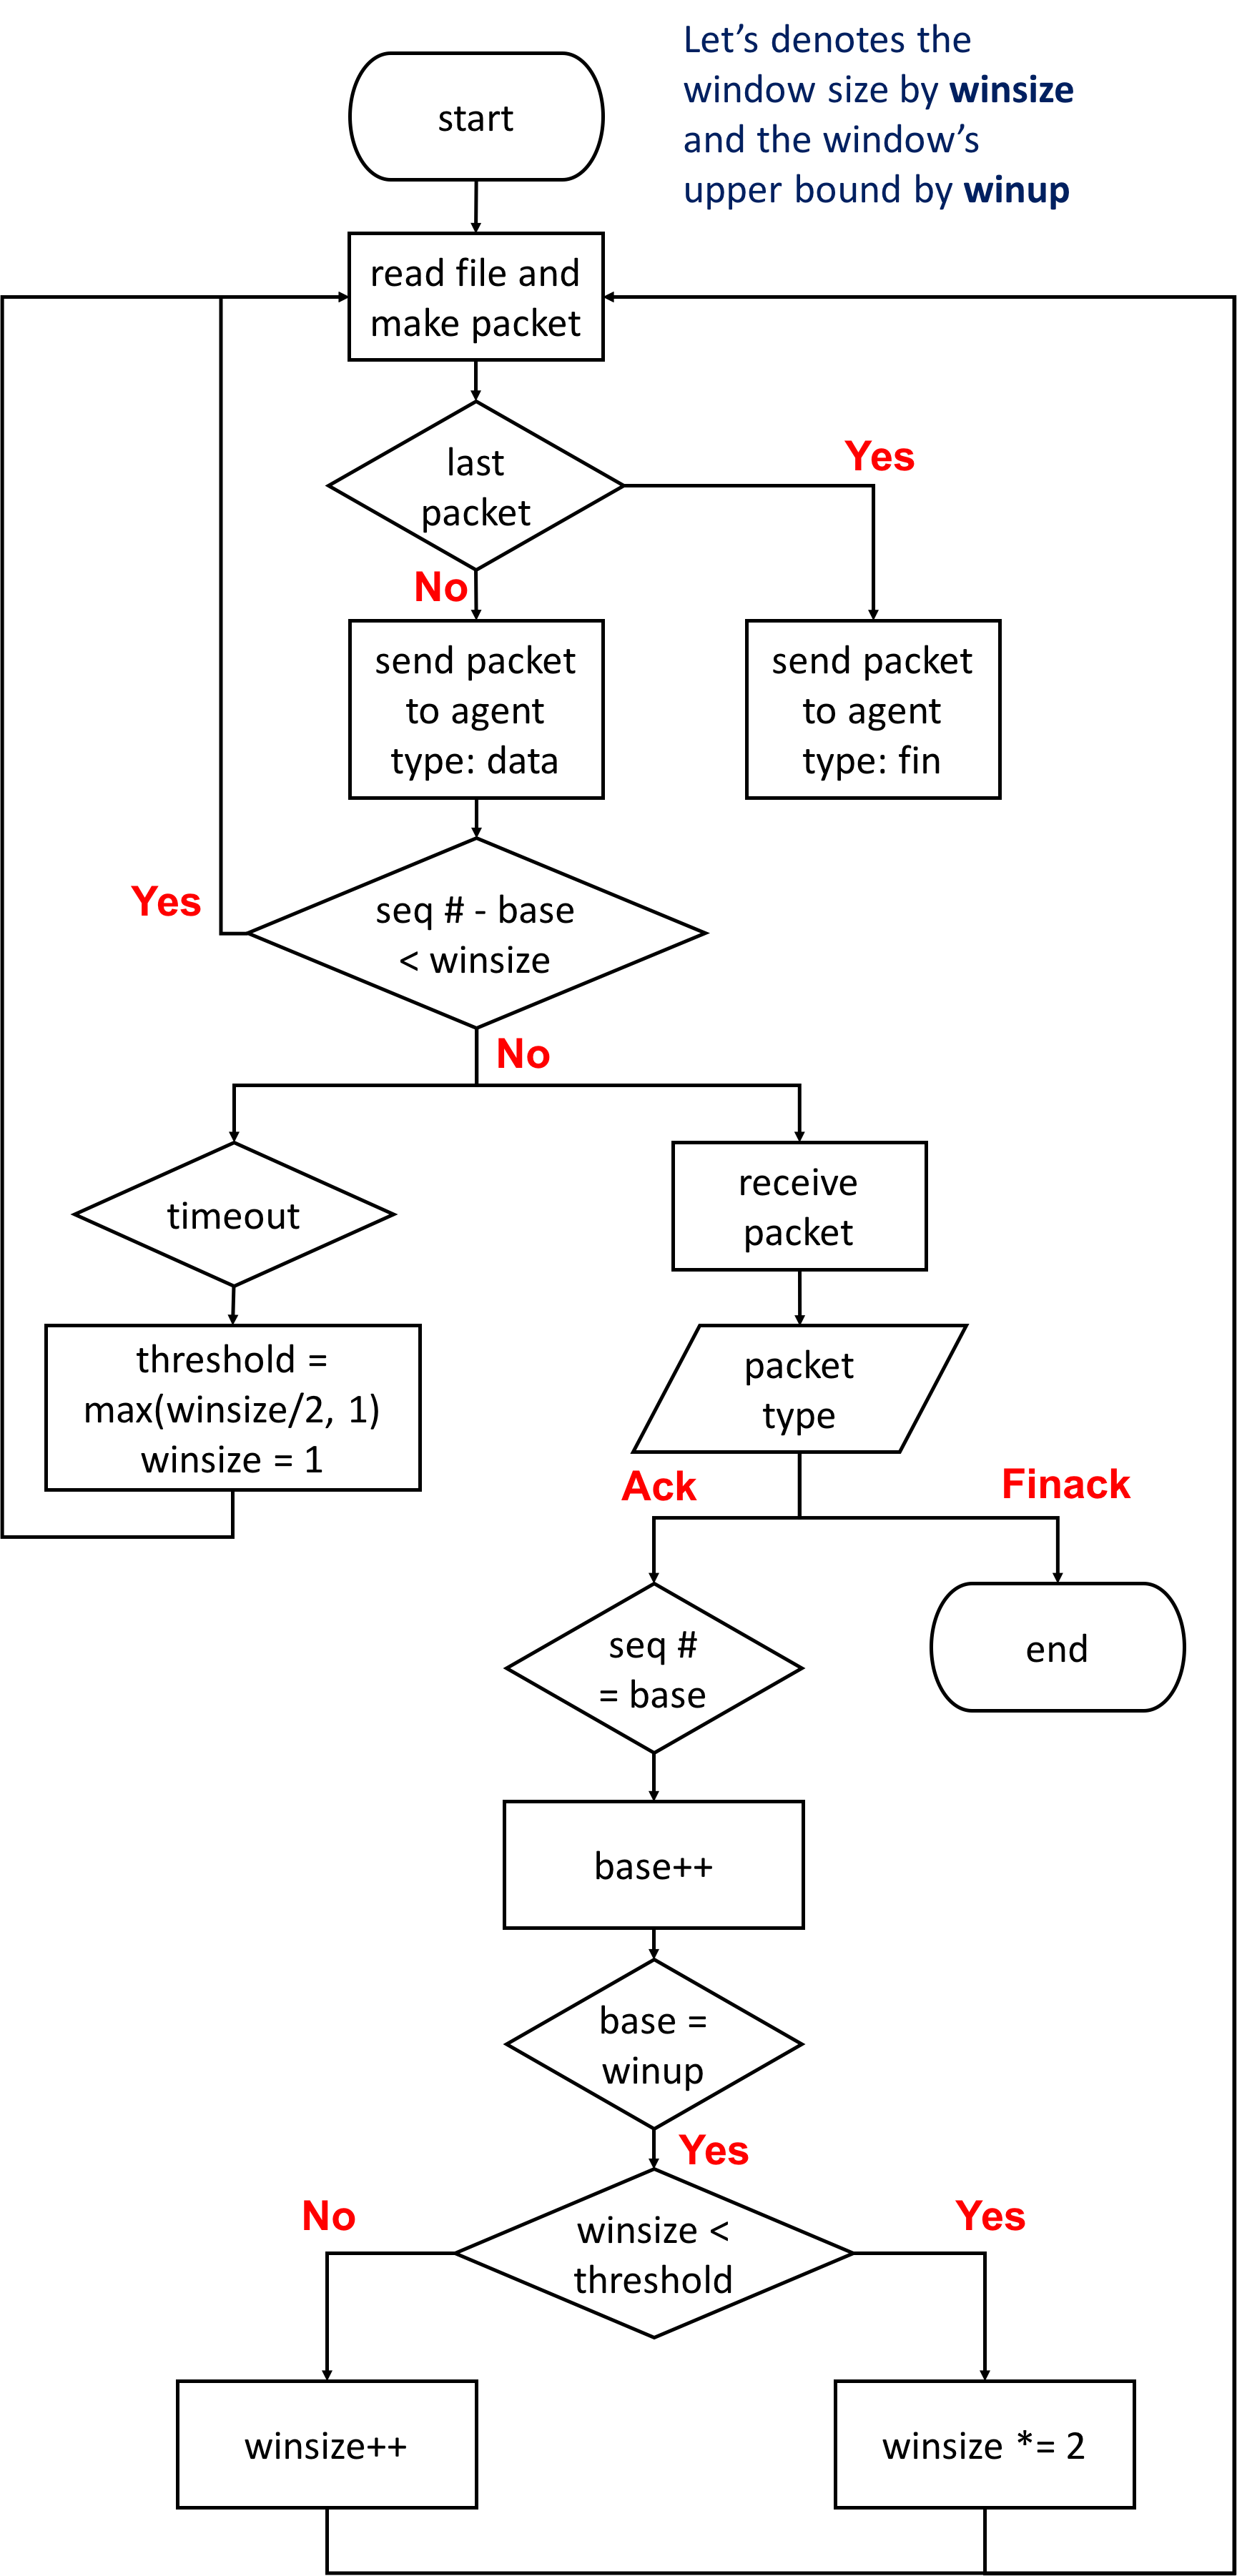
\includegraphics[height=23cm, keepaspectratio=true]{sender.png}
		\subsection*{Agent}
			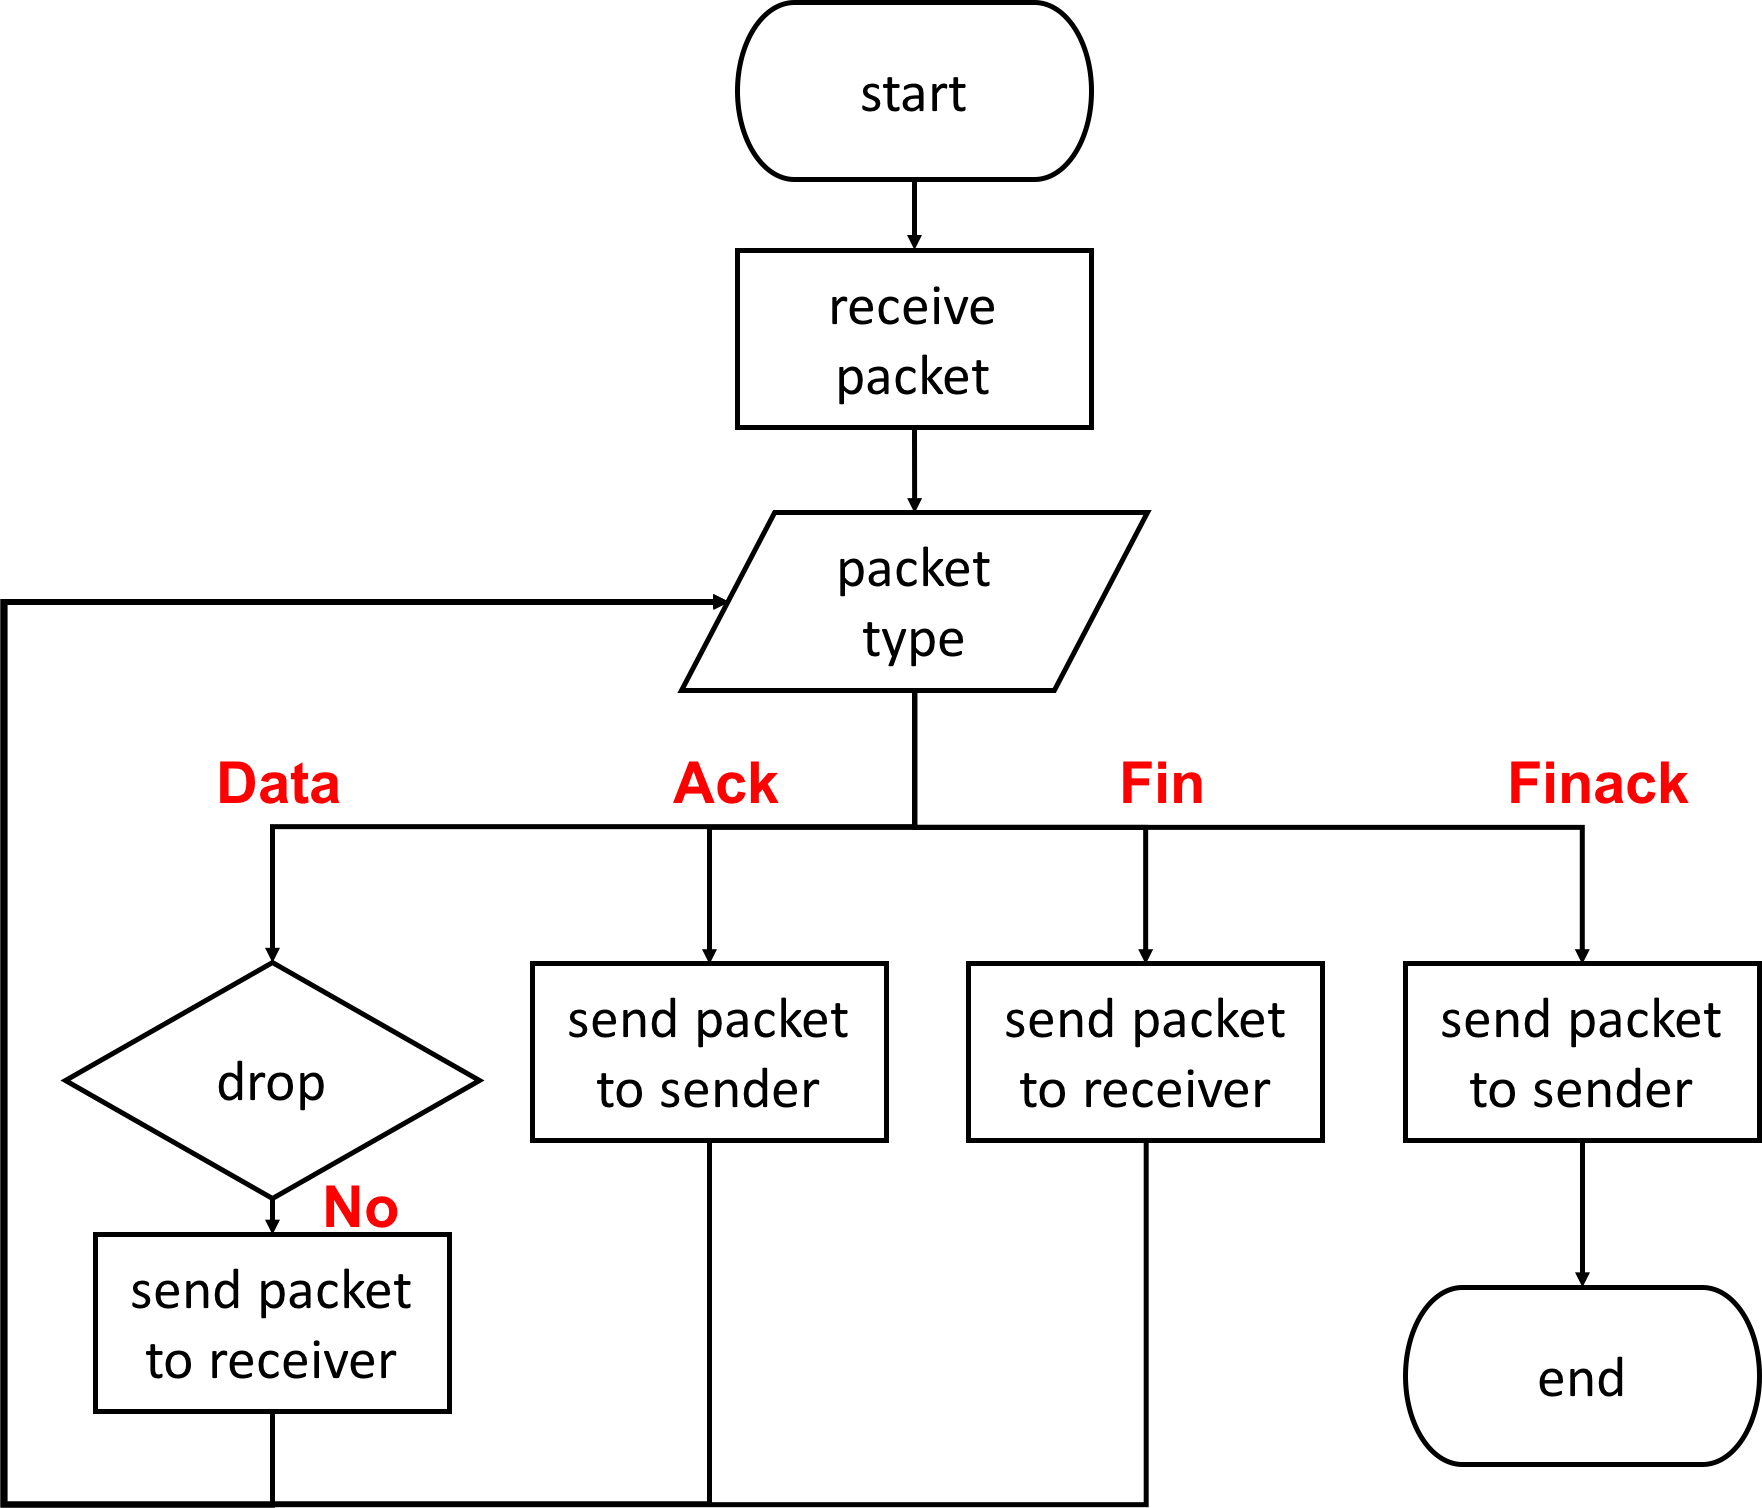
\includegraphics[height=11cm, keepaspectratio=true]{agent.png}
		\subsection*{Receiver}
			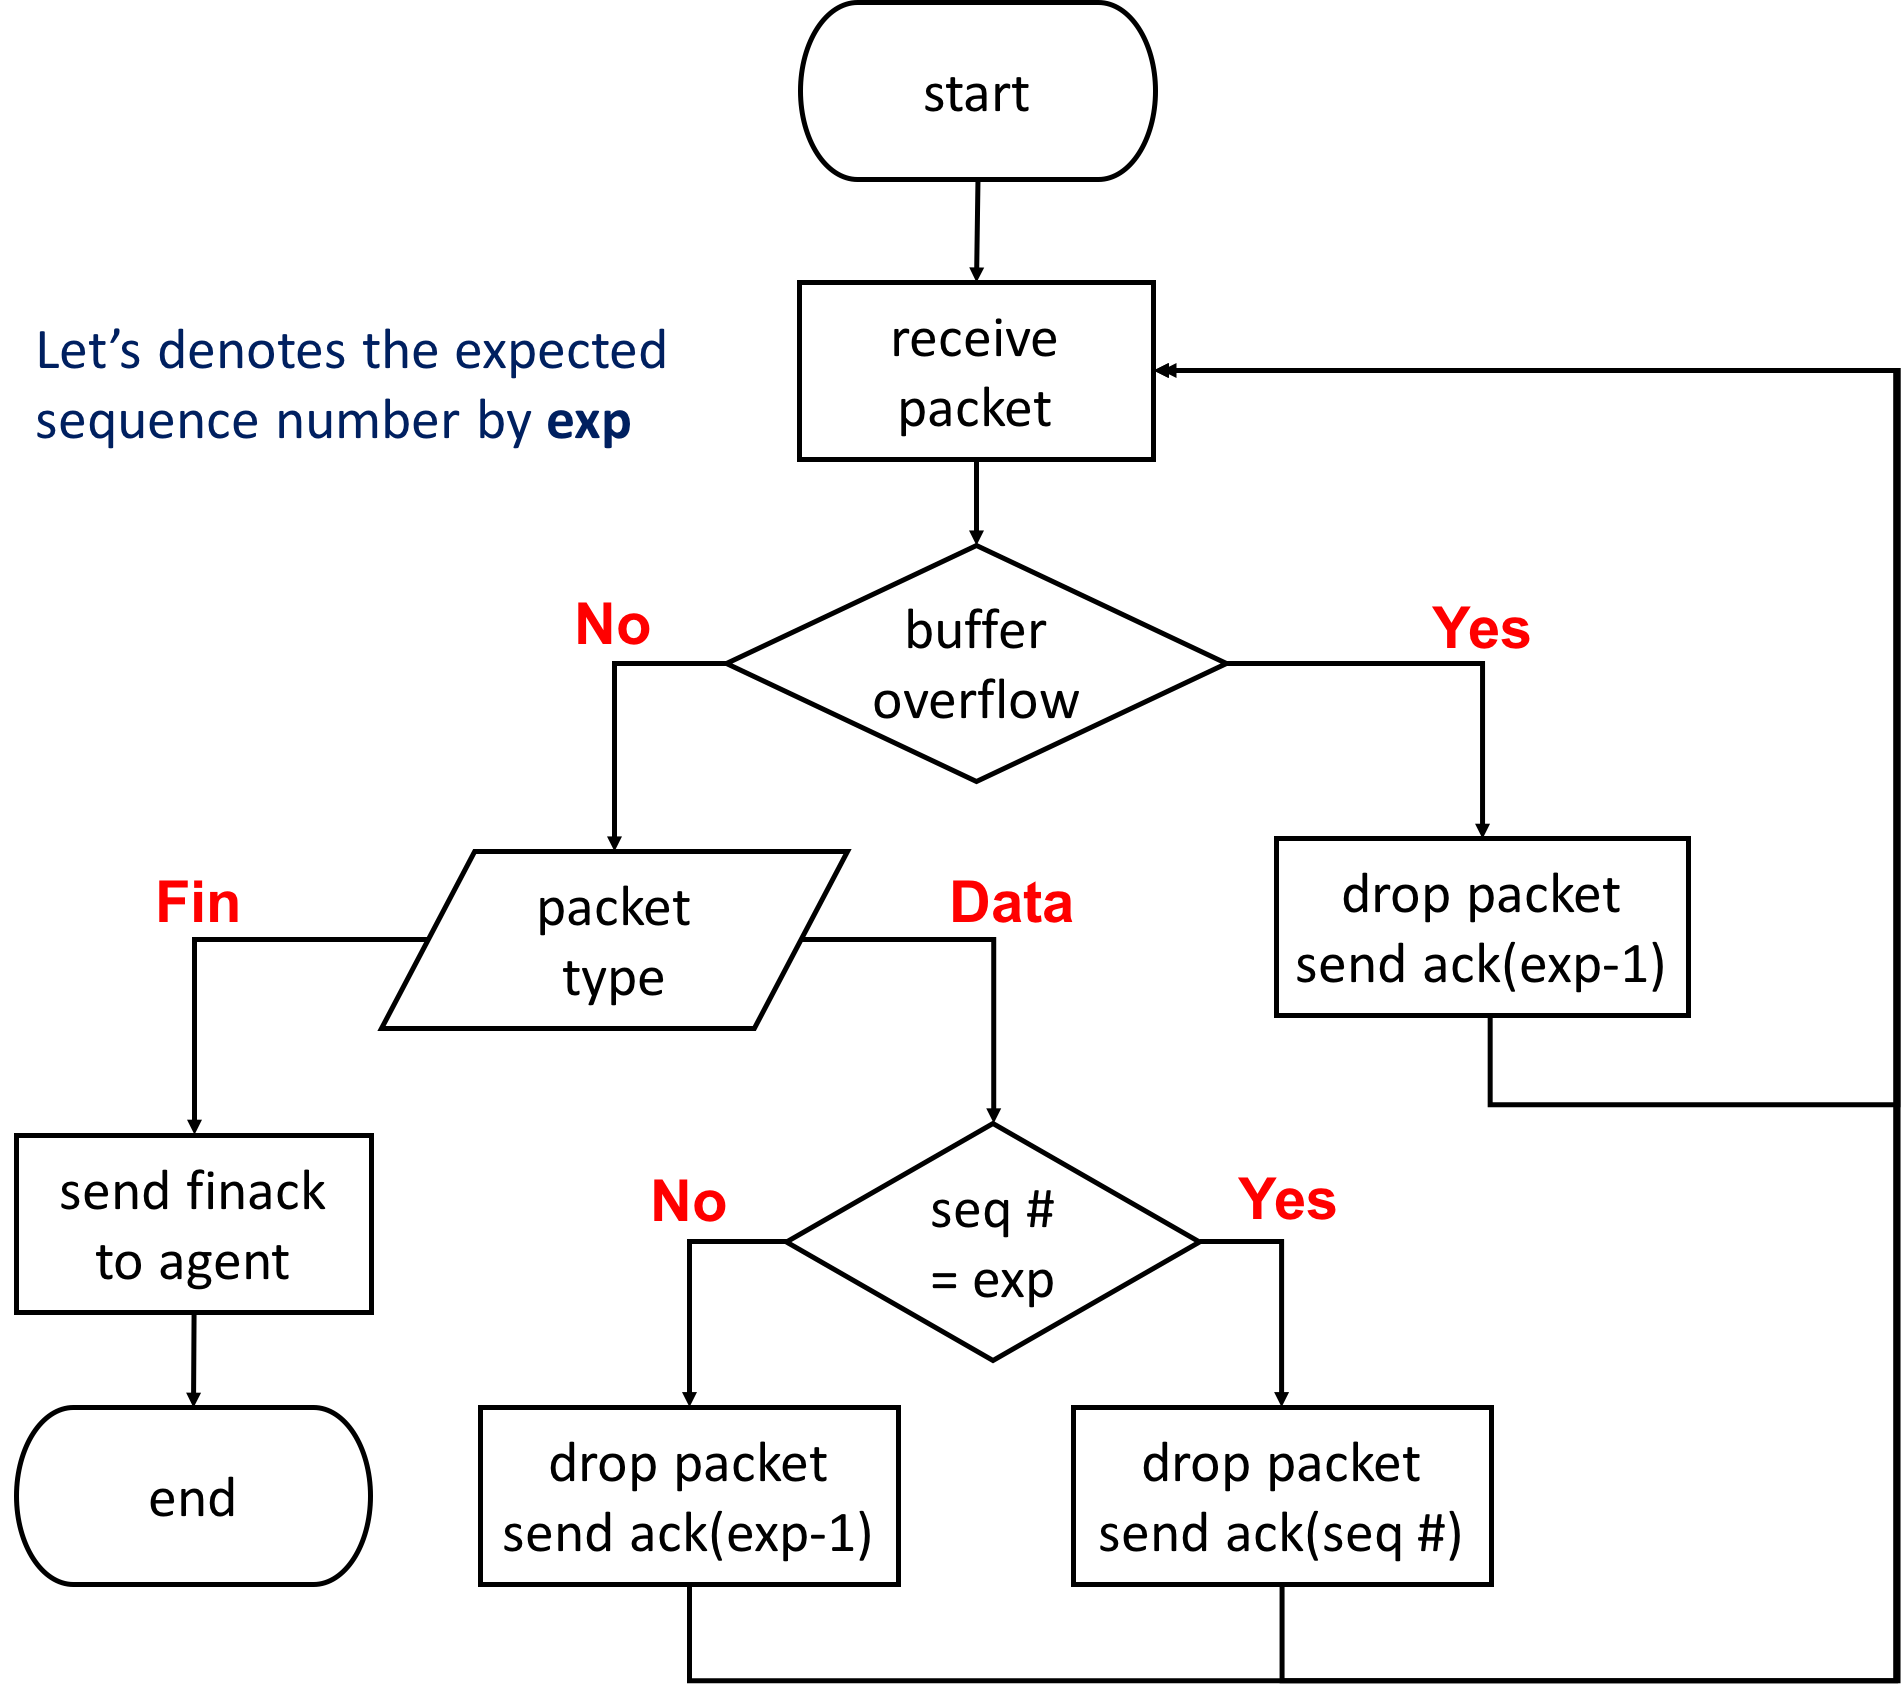
\includegraphics[height=11cm, keepaspectratio=true]{receiver.png}

	\section*{Difficulties \& Solutions}
		\begin{enumerate}
		\item
			Difficulty: Timeout for sender \\
			Soultion: Use select
		\item
			Difficulty: Buffer overflow for receiver \\
			Soultion: Record the number of packets received. When a packet is received and the buffer is full, flush the buffer and drop that packet.
		\end{enumerate}
	
	\clearpage
	\end{CJK}
\end{document}